\chapter{Become the Person Who Attracts Help}

On the road to wealth freedom, help is not a decorative topic. It is part of the machinery.

A person cannot build everything alone. Capital, knowledge, opportunity, trust, judgment, distribution, and courage all move through relationships. Sometimes the decisive resource arrives as a book, a teacher, a partner, an introduction, a warning, a sentence spoken at the right time, or a person who opens a door before we even understand that there is a door.

In ordinary language, such a person is often called a benefactor. The word may sound old-fashioned, but the underlying phenomenon is practical: a benefactor is someone whose presence, advice, trust, resources, or example helps you move to a higher level.

The question is not merely, ``How do I find such people?'' That question is too passive. It imagines the world as a lottery.

A better question is:

\begin{quote}
What kind of person repeatedly meets valuable help?
\end{quote}

The answer is simple enough to sound disappointing:

\begin{quote}
First become a benefactor yourself.
\end{quote}

Only then are you more likely to meet benefactors. More accurately, only then are you more likely to be noticed, trusted, helped, and pulled into value networks where such people naturally appear.

\section*{Serendipity Is Not Pure Luck}

Many people explain the repeated appearance of benefactors as luck. Some even reduce it to personality labels: high emotional intelligence, low emotional intelligence, cleverness, charm, likability, and so on. These labels often explain less than they appear to explain.

The deeper issue is not whether a person is charming. The deeper issue is whether that person is worth helping, easy to help, and visibly moving toward something that deserves help.

Serendipity looks accidental from the outside. A meeting happens, a conversation starts, someone offers advice, another person introduces a contact, a stranger becomes a teacher. Yet many so-called accidents are attracted by prior structure. If a person has been learning, producing, sharing, respecting others, asking clearly, and doing the right things for a long time, then a sudden opportunity is not pure chance. It is chance landing on prepared ground.

The person who receives help often appears lucky. But luck is not evenly attracted.

\begin{center}
\begin{adjustbox}{max width=\linewidth}
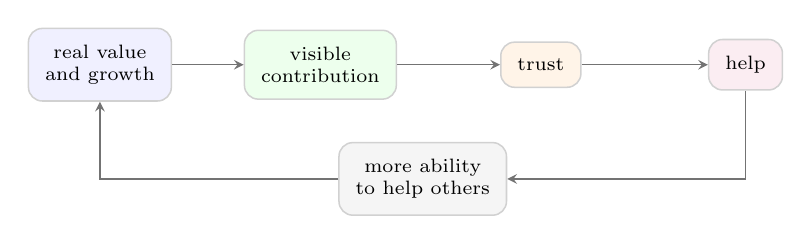
\begin{tikzpicture}[font=\scriptsize, line width=0.55pt, >=stealth]
  \node[draw=black!18, fill=blue!6, rounded corners=5pt, align=center, inner sep=6pt] (value) at (0,0) {real value\\and growth};
  \node[draw=black!18, fill=green!7, rounded corners=5pt, align=center, inner sep=6pt] (visible) at (2.8,0) {visible\\contribution};
  \node[draw=black!18, fill=orange!9, rounded corners=5pt, align=center, inner sep=6pt] (trust) at (5.6,0) {trust};
  \node[draw=black!18, fill=purple!7, rounded corners=5pt, align=center, inner sep=6pt] (help) at (8.2,0) {help};
  \node[draw=black!18, fill=gray!8, rounded corners=5pt, align=center, inner sep=6pt] (more) at (4.1,-1.45) {more ability\\to help others};
  \draw[->, draw=black!55] (value) -- (visible);
  \draw[->, draw=black!55] (visible) -- (trust);
  \draw[->, draw=black!55] (trust) -- (help);
  \draw[->, draw=black!55] (help) |- (more);
  \draw[->, draw=black!55] (more) -| (value);
\end{tikzpicture}
\end{adjustbox}
\end{center}

This loop is one reason wealth freedom is not only a private financial state. It requires a person to become the sort of node through which value can pass.

\section*{A Family Lesson}

In 1980, after years of political suffering and displacement, my father had a chance to go to Beijing to seek rehabilitation under the new policy environment. He had been teaching in a remote county in Heilongjiang. Before that, he had endured forced labor and the disorder of an era that damaged countless intellectuals.

The opportunity was real, but it was not secure. Many people had already gone to Beijing and had spent months waiting without result. My father hesitated. The family had little money. The journey itself was uncertain. There was no guarantee that the matter would be settled quickly, or at all.

My mother made the decision. She sold the house, used the deposit to buy the train ticket, and arranged for the family to stay temporarily at her workplace. Then she prepared my father carefully. She bought him clean clothes and told him to stand upright, speak clearly, and behave with dignity.

Her instruction became a family sentence:

\begin{quote}
We are not going there to complain about misery. We are going to ask for fairness. State the matter. Do not ramble.
\end{quote}

That sentence contains more wisdom than it first appears.

Many people in similar situations tried to make their suffering the main argument. They displayed injuries, hardship, and tragedy, as if greater misery should move them to the front of the line. Their pain was real. But pain alone does not necessarily make a request easier to handle.

My father did something different. He presented himself as clean, orderly, direct, and capable. He did not behave like a beggar. He behaved like a person with a legitimate matter to resolve. The result was striking. The process still required many stamps, queues, offices, and days of waiting. But again and again, people helped him. He returned after thirty-five days, one of the earliest and fastest successful cases in that place.

The lesson is not that clothing solves destiny. The lesson is that posture matters because it signals the nature of the interaction. Are you asking others to rescue a helpless burden, or are you inviting them to participate in a just and valuable correction?

Those are different requests.

\section*{Become Your Own Benefactor First}

My mother often said that she had met many benefactors in her life. Her explanation was plain:

\begin{quote}
You must first be a benefactor before you can meet benefactors.
\end{quote}

This is not moral decoration. It is an operational rule.

If you are useful, you can be connected to useful people. If you help others grow, people who care about growth are more likely to see you. If you share what you know, people who value knowledge are more likely to approach you. If you do not create unnecessary burdens, others are more willing to cooperate. If you are doing something right, people who recognize the right direction are more willing to add force.

The reverse is also true. If a person is always extracting, complaining, hiding, demanding, flattering, or waiting to be saved, valuable people learn to keep distance. They may be kind once. They will not build long-term trust.

A harsh but useful sentence follows:

\begin{quote}
If you are not growing, many forms of socializing are ineffective.
\end{quote}

The point is not to despise people who are still weak. Everyone begins weak somewhere. The point is that relationships built on real value require value to exist or to be visibly forming. Potential can attract help, but only if the potential is legible through action.

Even if a person meets no benefactor for a long time, the practice is still worthwhile. By trying to become a benefactor, the person grows. Eventually they discover that they have become the first reliable helper in their own life.

That helper will not easily leave.

\section*{The Right Thing Attracts Help}

The previous chapter described living in the future: using facts and logic to form a prediction, then acting before the future is obvious. This chapter adds a social consequence.

People who live in the future are easier to help, because others can see a future in them.

A person who is merely busy may be hard to help. There is activity, but no direction. A person who is merely ambitious may also be hard to help. There is desire, but no structure. A person who is doing the right thing, however, creates a different signal. Even if the work is unfinished, the direction is visible.

This connects to one of the most important rules in the whole book:

\begin{quote}
Doing the right thing is far more important than doing things right.
\end{quote}

Efficiency magnifies direction. If the direction is wrong, higher efficiency only creates a larger error. If the direction is right, even imperfect execution can accumulate.

This is why some plain principles are worth thinking through again and again. If a principle was true in the past, remains true now, and depends on durable features of reality, then it is likely to remain true in the future unless something extreme changes. Such principles allow us to live partly in the future.

For example:

\begin{itemize}
\item Knowledge compounds.
\item Attention is more valuable than noise.
\item Contribution attracts valuation over time.
\item Trust lowers the cost of cooperation.
\item Doing the right thing beats polishing the wrong thing.
\end{itemize}

These statements are easy to repeat and hard to live by. The difficulty is not pronunciation. The difficulty is conviction. Conviction requires thought, patience, and repeated action.

Many people are blocked less by ability than by wrong concepts. Change the concept, and the body may finally move.

\section*{Small Corrections in Language}

Some concept errors hide inside ordinary words.

A person says, ``I failed,'' and the sentence becomes a wall. Another person says, ``I am temporarily unsuccessful,'' and the same event becomes a stage in a longer process.

A person says, ``I hate this,'' and the mind closes. Another says, ``I have not learned to like this yet,'' and a small opening remains.

These are not childish tricks. They are operating-system patches. The mind acts according to the meanings it accepts. If every setback is final failure, patience disappears. If every discomfort becomes hatred, feedback becomes impossible to use. If asking for help means begging, cooperation becomes shameful. If receiving help means permanent debt, growth becomes burdened by anxiety.

The road to wealth freedom requires many technical skills, but it also requires cleaner concepts. A dirty concept makes clean action difficult.

\section*{Principles for Meeting Benefactors}

The following principles are not profound because they are obscure. They are profound because they remain true after repeated testing.

\begin{enumerate}
\item Optimistic people are more likely to become benefactors to others.
\item Benefactors are more likely to meet other benefactors.
\item A true benefactor helps others make progress, not merely feel comforted.
\item People who are excellent, reliable, and worthy of respect are easier to help.
\item People who share generously are easier to help.
\item People who do not create unnecessary burdens are easier to help.
\item People who are not ashamed to ask for help are easier to help.
\item When asking for help, money should not be the only imagined return.
\item When helping others, money should not always be collected as the return.
\item A powerful person is not necessarily a benefactor; some powerful people are only powerful for themselves.
\item Many successes happen because many people wish to see that person succeed.
\item Many failures are made heavier because many people do not wish to see that person succeed.
\item People doing the right thing receive more help.
\item People living in the future attract help because others can see possibility in them.
\end{enumerate}

The list can keep growing. But the center is stable: become valuable, become contributive, become easy to help, and become patient enough for the result to appear.

Most people cannot wait. They try a principle for weeks, find no miracle, and abandon it. But relationship value compounds slowly at first and then suddenly becomes visible. The curve is quiet for a long time before it rises.

\begin{center}
\begin{adjustbox}{max width=\linewidth}
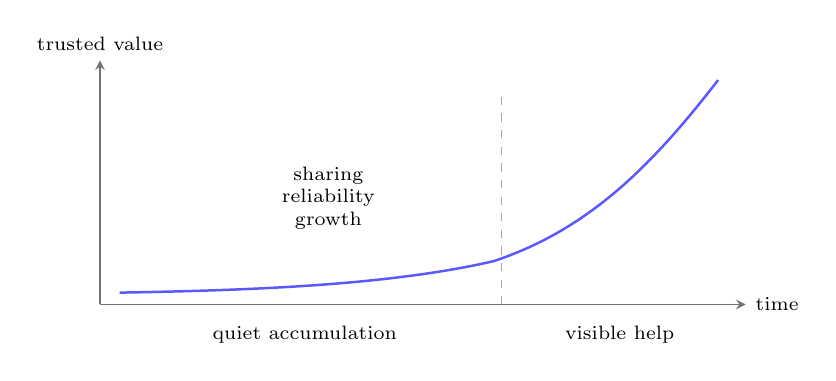
\begin{tikzpicture}[font=\scriptsize, line width=0.55pt, >=stealth]
  \draw[->, draw=black!55] (0,0) -- (8.2,0) node[right]{time};
  \draw[->, draw=black!55] (0,0) -- (0,3.1) node[above]{trusted value};
  \draw[draw=blue!65, line width=0.9pt]
    (0.25,0.15) .. controls (2.0,0.18) and (3.7,0.25) .. (5.0,0.55)
    .. controls (6.2,0.95) and (7.0,1.75) .. (7.85,2.85);
  \draw[dashed, draw=black!35] (5.1,0) -- (5.1,2.7);
  \node[align=center, anchor=north] at (2.6,-0.15) {quiet accumulation};
  \node[align=center, anchor=north] at (6.6,-0.15) {visible help};
  \node[align=center] at (2.9,1.35) {sharing\\reliability\\growth};
\end{tikzpicture}
\end{adjustbox}
\end{center}

Faith plus patience makes it possible to endure accidental disappointment long enough to meet inevitable good fortune.

\section*{Asking for Help Is Not Begging}

Many people misunderstand help because they misunderstand asking.

They imagine asking for help as lowering the head, flattering, pleading, smiling falsely, and making oneself small. That is not asking for help. That is begging.

A clear request for help is different. It has dignity, context, and value. It does not hide the difficulty, but it also does not dump the difficulty onto another person. It shows what has already been done, what is missing, why the matter is worth solving, and what kind of help would make a real difference.

To understand the concept, it helps to separate four different actions:

\begin{center}
\begin{adjustbox}{max width=\linewidth}
\begin{tabular}{p{0.22\linewidth} p{0.66\linewidth}}
\hline
\textbf{Action} & \textbf{Meaning} \\
\hline
Asking for help & Inviting another person to join a valuable process where their input can create progress. \\
Begging & Trying to obtain rescue mainly through pity or pressure. \\
Creating burden & Transferring disorder to someone else without preparation or respect. \\
Taking advantage & Using another person's resources mainly to reduce one's own cost while offering little value. \\
\hline
\end{tabular}
\end{adjustbox}
\end{center}

Asking for help is not the same as troubling others. When another person asks you for help, they may not be troubling you either. If the request is meaningful, clear, and connected to growth, helping can also help the helper.

This is easy to understand if you have ever helped someone seriously. At the moment you help, you may already receive a return. You confirm your own value. You clarify your own knowledge. You participate in another person's progress. You help build a future in which a capable person may later help others, including you.

The return is not always immediate, monetary, or measurable. But it can still be real.

\section*{Help Is a Hidden Transaction}

Every person lives inside exchanges of value. The modern world increasingly resembles a vast market, not only for goods and money, but also for attention, trust, reputation, knowledge, and opportunity.

Smart people therefore do two things almost instinctively:

\begin{enumerate}
\item They store interpersonal value.
\item They move toward clusters with high interpersonal value.
\end{enumerate}

Storing interpersonal value does not mean manipulating people. It means becoming the kind of person whose presence lowers costs, increases clarity, improves outcomes, and makes cooperation pleasant. Moving toward high-value clusters means spending more time where people learn, build, share, keep promises, and care about long-term results.

From this angle, asking for help is not the art of flattery. It is the art of presenting value correctly.

A benefactor helps because some value is already visible. Perhaps helping you confirms their own value. Perhaps your growth gives them satisfaction. Perhaps they see a future possibility that you cannot yet fully see. Perhaps your work serves a direction they also believe in. The reason may not be explicit, but value is almost always involved.

This is why money is often a poor immediate return for help. In some situations, payment is proper. Professional service should be paid for. But many acts of help belong to a wider exchange. If every act is priced immediately, the relationship becomes smaller than it needs to be. If every act is treated as a favor that can never be repaid, the relationship becomes heavier than it needs to be.

A better model is delayed and distributed exchange. You receive help now. You grow. Later you help the same person, or someone they care about, or another person on the same road. Value continues moving.

\section*{The Anxiety of Owing}

When we have not yet produced much, receiving help can feel uncomfortable. It may feel as if we owe a debt we cannot repay.

This anxiety is normal, but it can become another wrong concept. If you interpret help only as personal debt, you may become trapped by shame. You may avoid asking. You may waste the help by worrying about repayment instead of growing into the kind of person who can repay value later.

Add one word:

\begin{quote}
Temporarily.
\end{quote}

You are temporarily unable to repay. You are temporarily short of resources. You are temporarily inexperienced. You are temporarily dependent on another person's trust.

That word changes the structure. It does not erase responsibility. It makes responsibility bearable. The proper response to help is not lifelong guilt. The proper response is growth.

Trust the benefactor's judgment. If someone chooses to help you, perhaps they see something. Perhaps they believe that with time you will become capable. Perhaps they are investing in a future version of you. Your task is to make that judgment less wrong.

\section*{How to Become Easier to Help}

A practical request for help should pass several tests.

\begin{enumerate}
\item Have you tried seriously before asking?
\item Can you describe the problem clearly?
\item Can you show why the matter is worth solving?
\item Can you ask for a specific kind of help rather than vague rescue?
\item Can you reduce the helper's burden by preparing context?
\item Can you accept feedback without defending your ego?
\item Can you report back after the help has produced results?
\end{enumerate}

The last point is often neglected. Reporting back is a form of respect. It closes a loop. It tells the helper that their attention was not wasted. It also makes future help more likely, because the helper can see progress.

A person who disappears after receiving help teaches others not to help again. A person who returns with progress teaches others that help given to them can compound.

\section*{Social Capital Before Financial Capital}

The next stage of this book will discuss capital more directly. Before that, it is useful to notice that benefactors are part of a broader form of capital.

Financial capital is stored purchasing power. Social capital is stored trust, contribution, reputation, access, and goodwill. It cannot replace money in every situation, but it can create paths that money alone cannot buy.

Like financial capital, social capital can be wasted. It is wasted by dishonesty, unreliability, arrogance, greed, vague requests, emotional disorder, and repeated extraction. It is built by contribution, clarity, patience, competence, fairness, and the willingness to help others progress.

The person seeking wealth freedom should therefore stop treating relationships as decoration. Relationships are not merely entertainment, comfort, or status. They are part of the infrastructure through which future value moves.

But the order matters. Do not chase benefactors. Become someone worth helping. Do not collect contacts. Build value. Do not worship powerful people. Move toward people who help progress happen.

A powerful person may only be powerful. A benefactor makes others more capable.

\section*{A Practice for This Chapter}

First, write down the benefactors you have met. For each one, answer:

\begin{itemize}
\item What did they help me see, obtain, correct, or become?
\item Why were they willing to help?
\item What value, however small, had I already shown?
\item Did I report back, grow, or pass the value onward?
\end{itemize}

Second, write down the people for whom you have been a benefactor. Do not count only dramatic rescues. Count useful introductions, clear explanations, patient correction, shared knowledge, encouragement joined to standards, and moments when you helped another person make progress.

Third, choose one person you can help this week without creating dependency. The goal is not to perform kindness. The goal is to help progress occur.

Finally, identify one request you have been avoiding because you confuse asking with begging. Rewrite it with dignity. State the situation, what you have already done, what you need, why it matters, and how you will use the help responsibly.

\section*{The Mirror}

Meeting benefactors is partly accidental and partly inevitable. It is accidental because no one controls timing, location, and every human choice. It is inevitable because a person's life becomes a mirror. Over time, the mirror reflects the kind of person they are becoming.

If you are optimistic, useful, respectful, contributive, clear, patient, and future-oriented, more people will want to see you succeed. If many people want to see you succeed, help appears more often. If help appears more often and you use it well, your growth accelerates. If your growth accelerates, you can help more people.

This is not a trick. It is a compounding process.

The road to wealth freedom is walked by individuals, but it is not walked alone. The best way to meet benefactors is to become one. Then, even before the next helper appears, the path has already changed: you are no longer waiting for rescue. You have become a source of value.
